\section{Motivation}

Die Welt ist auf dem Weg in das Web 3.0, die Unternehmen wechseln zur Industrie 4.0 und die Cloud kommt demnächst in Version 2.0. Was am Ende bleibt sind Technologien die sich gegenüber anderen Technologien bewährt haben. Zum Einen durch ihren Mehrwert in der Forschung und zum Anderen durch ihren praktischen Nutzen im breiten Feld.\\
Eine Technologie die bereits heute eine viel zahl von neuen innovativen Ideen im privaten Sektor hervorgebracht hat, erobert den industriellen Sektor - Blockchain. So erwägen einige der größten Finanzinstitutionen den Einsatz eines Distributed Ledgers.\cite{Goldman2018}\cite{JPMorgan2018}\\

“Es ist davon auszugehen, dass wir in ein bis zwei Jahrzehnten wirtschaftlich über Mechanismen miteinander interagieren werden, für die wir bislang weder Konzepte noch Begriffe haben.”\cite[S.~92]{Platzer2014} Selbst die Deutsche Bundesregierung ist an der Blockchain Technologie interessiert und erwägt den Einsatz in der Zukunft für die unterschiedlichsten Services. In einer der jüngsten Pressemitteilungen hat der Blockchain Bundesverband mitgeteilt, dass die Regierung eine umfassende Strategie zum Umgang und Einsatz der Technologie erarbeiten will.\cite{BCBundesverband2018}

\begin{figure}[h!]
	\centering
	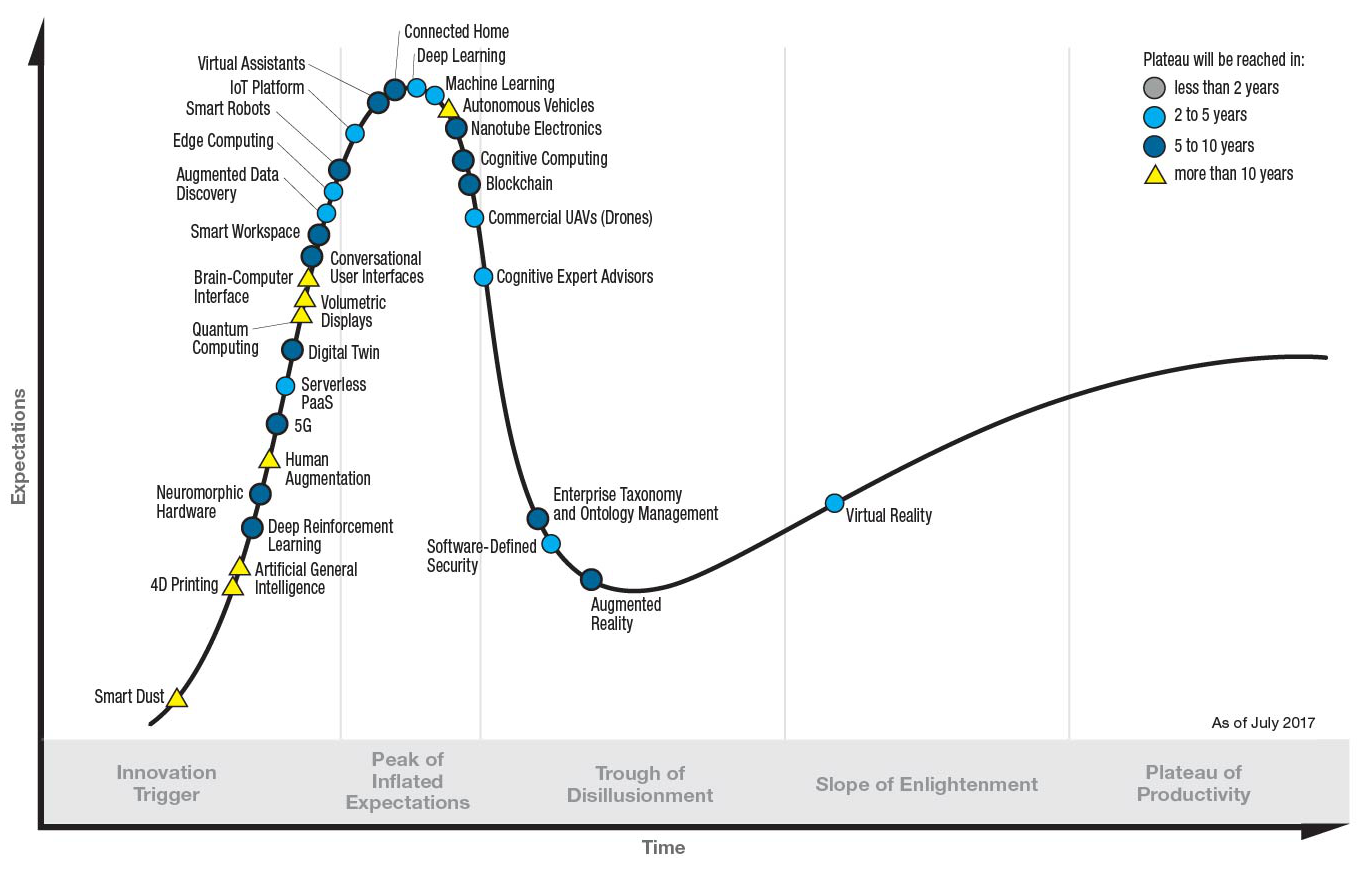
\includegraphics[width=0.79\linewidth]{pictures/Gartner-Hype-Cycle-2017}
	\caption[Gartner Hype Cycle 2017]{Emerging Technologies Hype Cycle 2017\cite{Gartner2017}}
	\label{fig:gartner-hype-cycle-2017}
\end{figure}

Noch ist die Blockchain kein Alltag. Bemessen am jährlich erscheinenden Hype Cycle des Marktforschungsinstituts Gartner, Inc. $( Abb.~ \ref{fig:gartner-hype-cycle-2017} )$ hat die Technologie noch fünf bis zehn Jahre Entwicklungszeit vor sich. Erst dann wird sie nach aktueller Einschätzung im produktiven Einsatz sein. Was der Hype Cycle nicht aussagt ist welchen Einfluss die Blockchain auf eine Branche oder die Gesellschaft hat in ihrer jeweiligen Phase.\\

Bereits heute zeigen sich signifikante Unterschiede zwischen den unzähligen Blockchains die in Pilotprojekten realisiert wurden. So gibt es Anwendungen der Blockchain um beispielsweise den Kilometerstand eines Fahrzeugs täglich \glqq in die Blockchain\grqq~ zu schreiben. Der Nutzen liegt klar auf der Hand. Die inhärenten Eigenschaften der Blockchain ermöglichen es sehr einfach festzustellen, ob ein Kilometerstand nachträglich durch Fremdeinwirkung manipuliert wurde. Ebenfalls ist keine zentrale Zwischenstelle mehr nötig, um für die Echtheit des hinterlegten Wertes zu garantieren.\cite{carVertical}\\

Bitcoin war die erste Generation von Blockchain. Ethereum war die zweite und mittlerweile behaupten die ersten Projekte von sich zu der dritten Generation von Blockchains zu gehören. Skalierbarkeit und Interoperabilität spielen in dieser Generation eine der entscheidenden Rollen.\cite[vgl.]{Cardano} Auch die Blockchain Anwendungen im Enterprise Bereich lassen in Masse noch auf sich warten. Es fehlen Erfahrungen und konkrete Einsatzgebiete für die Technologie.

\newpage